%导言段 定义纸大小 引入模版 中文支持 页边距设置 页眉页脚设置
\documentclass[a4paper]{ctexrep}
\usepackage{xeCJK,geometry,fancyhdr,abstract,graphicx}
	%宋体
	\setCJKmainfont{SimSun} 
	\geometry{left=2.7cm,right=2.7cm,top=3.5cm,bottom=2.5cm} %页边距
	\CTEXsetup[number={\arabic{chapter}}]{chapter}
	%设置首页 不加时间
	\title{基于OVAL的漏洞管理与发现系统}
	\author{夏映晖}
	\date{}
	%设置页眉页脚
	\pagestyle{fancy}
	\lhead{}
	\chead{北京理工大学工程硕士学位论文}
	\rhead{}
	\renewcommand{\headrulewidth}{0.5pt}
	%使含有Chapter页面不清除页眉页脚
	\fancypagestyle{plain}{}

%文档开始
\begin{document}
	%%%%%%%%%%%%%%%%%%%%%%%%%%%%%%%%%%%%%%%%%%%%
	%首页
	\maketitle
	%中文摘要
	\begin{abstract}
	漏洞管理系统需要具有与网络漏洞库实时同步、于本地系统高效扫描等特性。本文以一种开放漏洞描述语言OVAL为基础,构建了能满足高效同步、扫描的开放漏洞管理系统,能够在任何CVE条目更新时发现本地漏洞,并使用XBase作为XML数据库,从而对半结构化的漏洞数据进行高效管理。并且本系统以OVAL为基础实现了漏洞检查,比OVAL本身实现的系统检查时间减少50\%。另外,以该系统为核心,本文又进行了漏洞发生模式的预测,可为信息安全管理提供安全策略优先级建议。
	
	关键词:漏洞管理;OVAL;CVE;漏洞预测
	\end{abstract}
	%英文摘要
	\renewcommand\abstractname{abstract}
	\begin{abstract}
	TBD.
	
	Key Words: TBD.
	\end{abstract}
	%目录页
	\tableofcontents
	%新页 计页数
	\newpage
	\setcounter{page}{1}
	%%%%%%%%%%%%%%%%%%%%%%%%%%%%%%%%%%%%%%%%%%%%
	%第一章
	\chapter{绪论}
		%第一节
		\section{研究背景和意义}
		漏洞发现的方法研究有很多,如,静态分析测试、模糊测试、基于属性的安全测试、形式化安全测试、基于渗透的安全测试等。这些方法利用了不同的安全理论和技术,从不同的角度对软件安全性测试做出了探讨,有较多差异性。
		
		从理论的形成思想可以将这些方法分为基于系统性考虑的方法以及基于有效性考虑的方法,前者重于通过模型或知识库充分地遍历软件状态,扫描可知的安全性漏洞,但无法避免效率低、误报率高的缺点;后者重于有效地发掘软件漏洞,常常可以发现未知的安全性漏洞,但局限性较大、漏报率高、不够全面和系统。

		近年来,由于软件规模的增大,设计模式的多样化,测试人员很难从架构和设计中找到更多安全性漏洞,系统性的方法效率不高,因此以模糊测试为代表的完全自动化方法逐渐流行起来,成为了攻防两端都会关注的方法。此外,由于已发现的漏洞规模增大,以此为依据构建的知识库也成为了发现新漏洞的有效工具。
		%第二节
		\section{国内外研究概况} 
		漏洞管理也是软件安全的重要课题。有多种漏洞形式化方法被提出,从语义网发展的本体方法是其中一种,Ju An Wang等人建立了一个基于本体技术的漏洞管理系统,能够从漏洞数据库中获取信息安全概念, 并可推理漏洞可能产生的影响。对于自动化漏洞管理上,Martín Barrère等人尝试利用OVAL增强Android实时安全性,实现了一个轻量级自动化漏洞评估系统;进一步地,他们针对漏洞生命周期提出了一个基于OVAL的预测模型,用于检测遗留系统的漏洞。XinMing Ou等人提出了MulVAL,旨在通过OVAL自动发现大规模网络中的漏洞,并可以与入侵检测系统形成互补。

		由于大规模数据分析近年来如火如荼,基于漏洞库的知识发现也成为学者们关注的焦点。Omar H. Alhazmi等人探讨了漏洞的量化特征的提取与漏洞预测的可能性,并在商业和开源系统中均通过逻辑或线性回归模型获得了收敛的结果。他们在另一篇文章中比较了Anderson等人提出的漏洞发现模型(VDMs),以及该模型之前Browne等人提出的漏洞发掘模型(VEMs),还有Alhazmi等人提出的Alhazmi-Malaiya Logistic Model(AML)等分布模型,并通过对现实数据的检测证明AML模型在漏洞记录较多的库中拥有较好性能。在VDMs之上,也有其他的研究,如Jinyoo Kim等人在多版本开源软件系统中挖掘漏洞,考虑了不同版本在同一软件上漏洞发现的影响,并用Apache和Mysql为例做了验证实验。Andy Ozement对VDMs等基于概率的模型提出了质疑,他认为VDMs在软件安全评估上拥有一定的好处,但即使拥有大量漏洞发现特征,该类模型在时间消耗、系统环境适配、漏洞发现独立性和静态代码依赖上都有一定的缺陷,因此VDMs仅能作为漏洞挖掘辅助系统。
		
		除了VDM相关研究外,机器学习在漏洞挖掘上也有其他维度的探讨,Mehran Bozorgi等人研究了系统管理中的漏洞防护优先问题,利用机器学习中的SVM分类器,可以预测漏洞是否发生、何时发生,与启发式专家知识系统相比拥有更好的准确性和补充性。同样应用了机器学习方法的辅助性自动软件漏洞检测有Fabian Yamaguchi等人提出的在代码级检测API使用模式的研究,也在真实环境下捕获了未知漏洞。
		%第三节
		\section{本文的主要工作}
		本文目标是基于OVAL描述语言构建漏洞管理及检测系统,在多种系统及软件版本下,分析系统环境条件自动检测已知漏洞,通过对知识库中大量CVE条目进行数据挖掘,可对未知的系统环境进行安全评估与漏洞预测。

		首先,本系统通过实时获取OVAL提供的CVE条目构建软件漏洞管理系统,利用协议信息得到漏洞检查语义,匹配系统环境及各软件的依赖逻辑关系,从而自动化发现系统中存在的已知漏洞。
		
		其次,通过对漏洞库的分析,抽取可用于分类未知软件漏洞的特征,使用机器学习的方法构造分类器来判断软件特定的模块可能产生的漏洞,并根据知识库得到该漏洞触发条件。并得到漏洞发生的优先序列,可用于系统的精益安全管理。
		%第四节
		\section{本文的组织结构}
		论文的结构和各章内容如下:
		
		第二章:探讨了漏洞管理相关理论与技术,对漏洞分类、基于OVAL的漏洞库设计以及CVE的管理模式进行了分析。
		
		第三章:研究了漏洞发生模式的挖掘技术,分别从先验角度和时间序列角度对漏洞发生模式进行讨论。
		
		第四章:阐述了本文中漏洞管理系统的设计与实现,并集成了漏洞挖掘及基于OVAL的漏洞库。

		第五章:阐述了本文中漏洞管理系统的测试工作。
		
		第六章:总结全文,分析系统中存在的问题,并探讨了未来工作。
	%%%%%%%%%%%%%%%%%%%%%%%%%%%%%%%%%%%%%%%%%%%%
	%第二章
	\chapter{漏洞管理相关理论与技术}
		\section{漏洞分类}
		漏洞可从成因、严重程度等角度进行分类,探讨目前存在的分类法
		\section{基于OVAL的漏洞库设计}
			\subsection{CVE的漏洞管理模式}
	%%%%%%%%%%%%%%%%%%%%%%%%%%%%%%%%%%%%%%%%%%%%
	%第三章
	\chapter{漏洞发生模式的挖掘}
		\section{条件先验知识下的漏洞发生模式挖掘}
			\subsection{算法描述}
			\subsection{实现}
		\section{时间序列上的漏洞发生模式挖掘}
			\subsection{算法描述}
			\subsection{实现}
	%%%%%%%%%%%%%%%%%%%%%%%%%%%%%%%%%%%%%%%%%%%%
	%第四章
	\chapter{漏洞管理系统的设计与实现}
		\section{需求分析}
			\subsection{功能需求}
			本系统包括以下几个主要功能模块:

			(1)漏洞展示模块:用于对漏洞的可视化展示,包括主页的可视化图及漏洞发生的日历

			(2)漏洞同步模块:实时同步并显示发生的漏洞

			(3)漏洞预测模块:从现有漏洞库中挖掘发生模式

			(4)漏洞管理模块:提供详尽的视图对漏洞进行增删改查

			(5)漏洞扫描模块:通过OVAL语言对本地系统进行检查

			(6)系统日志模块:记录本系统的任何行为

			(7)系统设置模块:设置本系统的各项参数配置

			\subsection{非功能需求}
			本系统需要实现以下几个主要非功能需求:

			(1)时效性:漏洞发生具有时效性,因此本系统也需要对新漏洞及时响应

			(2)兼容性:漏洞会在不同系统中发现,故系统需要满足跨平台特性

			(3)效率:系统拥有1秒内的漏洞查询性能、1分钟以下的漏洞检查性能

			(4)易用性:用户友好的界面、易学的操作

			(5)环境:运行于本地,可于本地对漏洞进行查询与检查

			\subsection{用例图}
			用户用例包括查看漏洞信息、查看漏洞预测、进行漏洞扫描、查看系统日志、设置管理系统等五个主要用例。在查看漏洞信息中,包括了查看漏洞趋势和查看漏洞统计两个子用例,并扩展了漏洞实时同步这个子用例,见图\ref{fig:1}。
				\begin{figure}[htb]
					\centering
					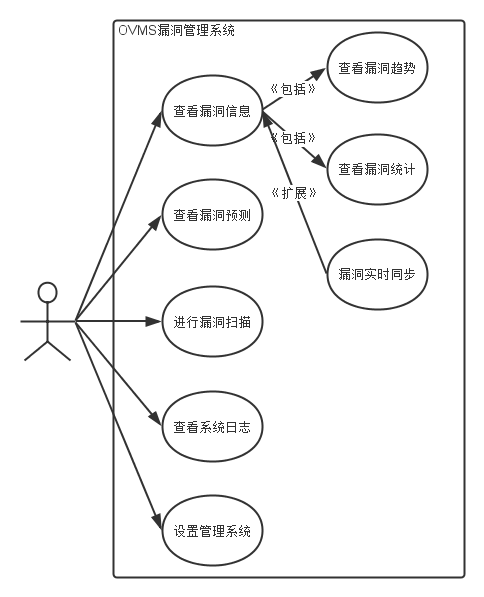
\includegraphics[height=10cm]{fig/1_usecase.png}
					\caption{\label{fig:1} 用例图}
				\end{figure}

		\section{系统设计}
			\subsection{系统架构图}
			\subsection{功能设计}
			\subsection{包图}
			\subsection{类图}
			\subsection{时序图}
			\subsection{ER图}
			\subsection{界面设计}

		\section{系统实现}
			\subsection{漏洞扫描模块的编写}
	%%%%%%%%%%%%%%%%%%%%%%%%%%%%%%%%%%%%%%%%%%%%
	%第五章
	\chapter{漏洞管理系统的测试}
		\section{单元测试}
			\subsection{具体模块单元测试编写}
		\section{系统测试}
			\subsection{功能测试}
			\subsection{非功能测试}
		\section{系统性能比较}
	%%%%%%%%%%%%%%%%%%%%%%%%%%%%%%%%%%%%%%%%%%%%
	%第六章
	\chapter{总结}
	对更多平台的适用性。与更多漏洞库进行同步。在漏洞发生模式预测上产生更好结果。
	%%%%%%%%%%%%%%%%%%%%%%%%%%%%%%%%%%%%%%%%%%%%
	%参考文献 unsrt引用顺序
	% \bibliographystyle{unsrt}
	% \bibliography{bitpaper}
	%文档结束
	\end{document}

